\section{Projektbeschreibung und Projektziele}
Für den praktischen Teil dieser Arbeit soll anhand der Entwicklung einer Ruby-on-Rails-Anwendung die Testgetriebene Entwicklung erkundet werden.

Als Ergänzung zu den lokalspezifischen Jobcommunitys mit strenger Mitgliederauswahl soll nun ein neues, allgemeines IT-Jobportal entwickelt werden. Der vorraussichtliche Name wird IT-Jobs-Und-Stellen.de\footnote{\url{http://www.it-jobs-und-stellen.de/}} sein.

Ziel soll es sein, eine konkurrenzfähige Alternative zu den Branchenprima stepstone.de, monster.de und jobscout24\footnote{
\url{http://www.stepstone.de} - \url{http://www.monster.de} - \url{http://www.jobscout24.de}} zu entwickeln. Folgende Kern-Anfordungen seien zu erfüllen


\begin{figure}[htbp]
 \centering
 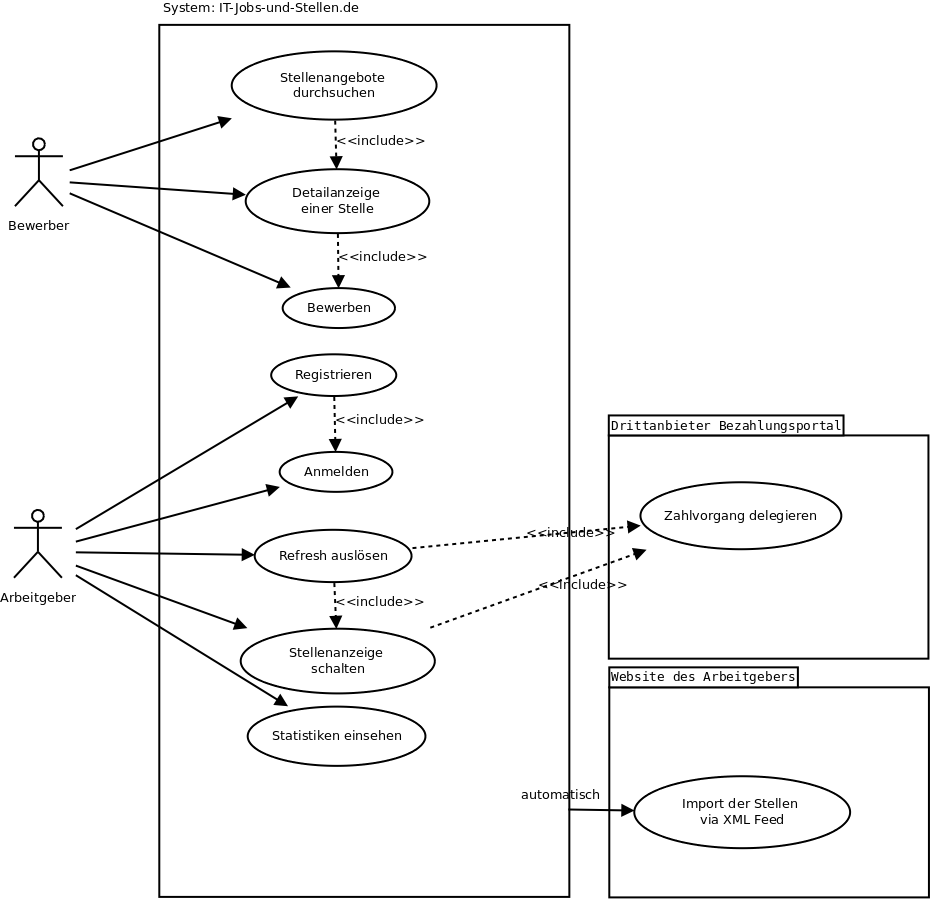
\includegraphics[width=1\textwidth]{./material/usecases.png}
 % usecases.png: 930x899 pixel, 51dpi, 46.50x44.95 cm, bb=
 \caption{Anwendungsfälle}
 \label{fig:usecases}
\end{figure}


\subsection{Funktionale Anforderungen}
\begin{itemize}
 \item Stellenanzeigen online schalten mittels eines Formulars
 \item Import von Stellenanzeigen mittels XML-Schnittstelle
 \item Eine möglichst einfache Handhabung sowohl durch Kunden als auch Bewerber
 \item Ein Bezahlsystem mit Einbindung eines 3rd Party Bezahldienstes zum Erwerb von Stellenanzeigen und Refreshs\footnote{Automatische Aktualisierung der Stellenanzeige und damit bessere Platzierung in den Suchergebnissen}
 \item eine Integration von Social Media Communitys, insbesondere Facebook, LinkedIn und XING, mit dem Ziel, den Bewerbungsprozess zu vereinfachen, z.B. um Lebensläufe generieren zu lassen
\end{itemize}

\subsection{Nichtfunktionale Anforderungen}

\begin{itemize}
 \item Eine hohe C0-Testabdeckung von mindestens 95\% als Grundlage für den TDD Prozess
 \item Eine hohe Erweiterbarkeit, um langfristig auch die bereits vorhandenen Jobcommunitys durch das neue System zu ersetzen, welche gegenwärtig auf Drupal 5 (PHP) basieren
 \item Eine moderne Suchfunktion durch einen Suchdaemon realisieren, z.B. Sphinx oder Lucene
 \item Softwarestack: Ruby 1.9.2 mit Ruby on Rails 3.1
\end{itemize}

